\section{Введение в эксперименты}

\begin{frame}{Пример - жульничество на выборах: \textcite{enikolopov2013field}}

\begin{itemize}
    \item Рандомизация независимых наблюдателей по 156
участкам из 3164 в Москве.
    \item Рандомизация – не «монеткой»/ «кубиком», а по
порядковому номеру участка.
    \item Однородные участки (исключены больницы и
военные части).
\end{itemize}


\end{frame}

\begin{frame}{Результат эксперимента}

\begin{figure}
    \centering
    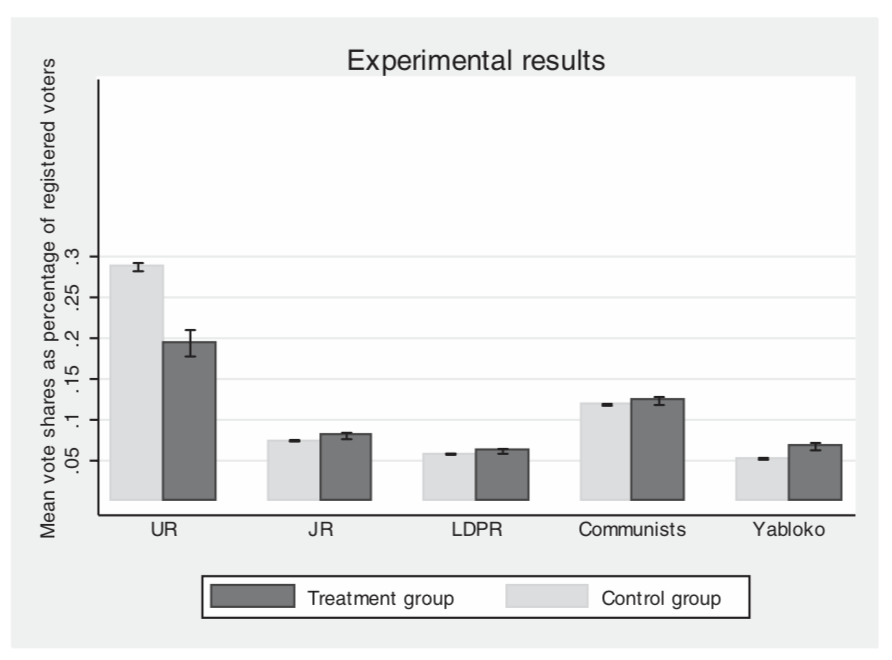
\includegraphics[width=\textwidth]{Images/main_result.png}
    \label{fig:my_label}
\end{figure}


\end{frame}


\begin{frame}{Пример гетерогенности - программа переселения из ветхого жилья в Чикаго: \textcite{chyn2018moved}}
\begin{itemize}
        \item Различия в судьбе детей из переселённых семей и оставшихся жить в неблагополучном районе. 
\end{itemize}
\begin{figure}
    \centering
    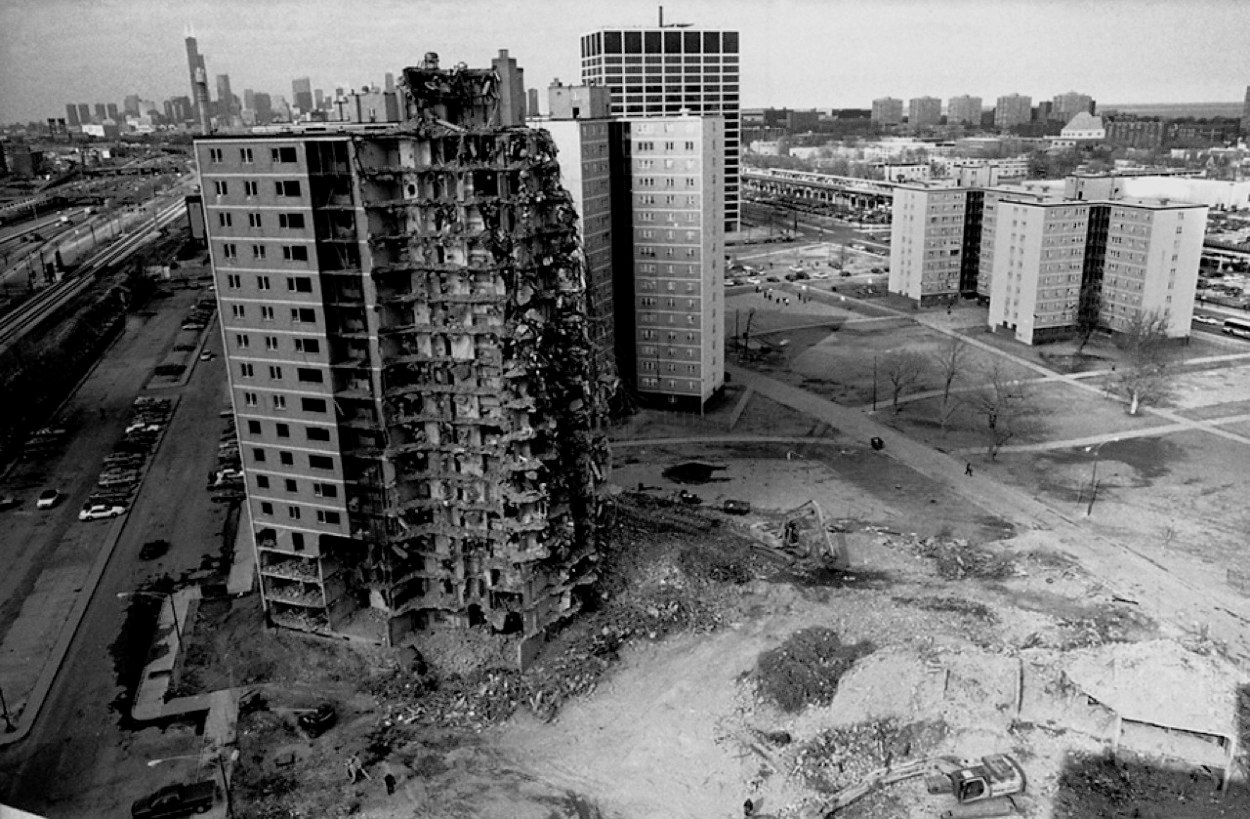
\includegraphics[width=\textwidth]{Images/Chicago_houses.jpg}
\end{figure}
\end{frame}

\begin{frame}{Эффекты для разных групп: \textcite{chyn2018moved}}
\begin{figure}
    \centering
    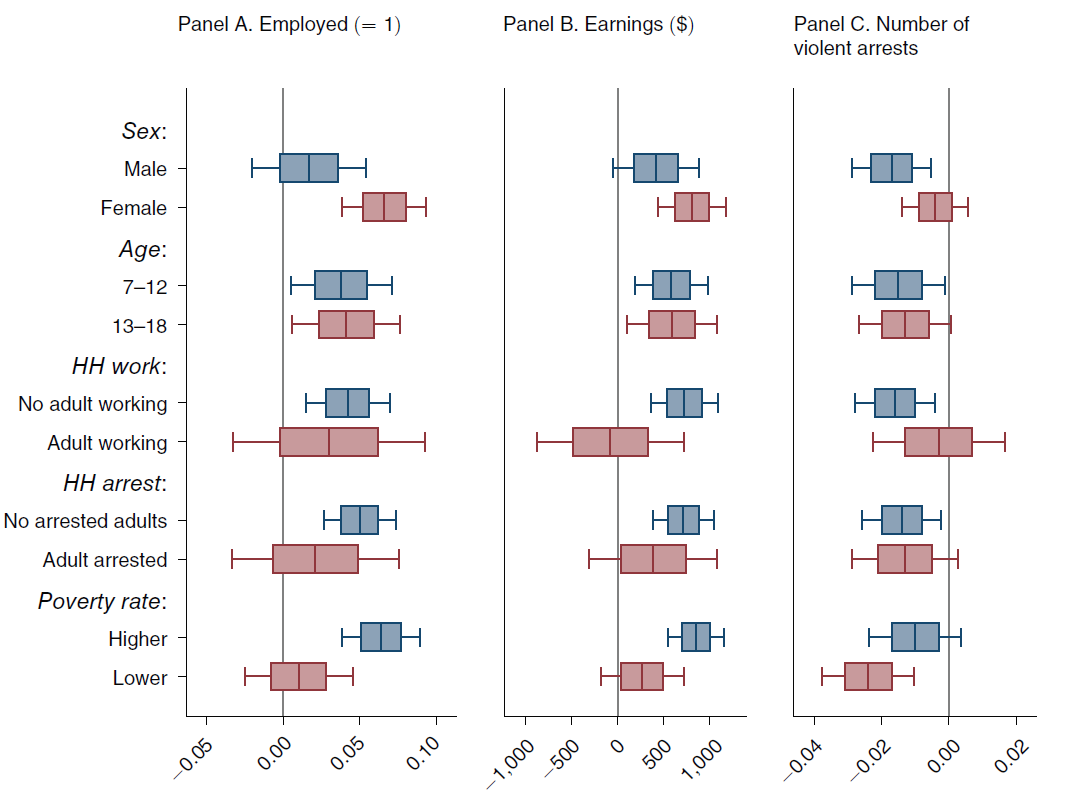
\includegraphics[width=\textwidth]{Images/Chicago2.png}
\end{figure}

 
\end{frame}
\begin{frame}{Примеры: что если нет эксперимента, но...}

\begin{itemize}
    \item Мы понимаем, от чего зависит назначение табетки
    \item Кандидат побеждает на выборах с 50.1 процентом голосов
    \item Не каждый, кому выдадут таблетку, ее примет
\end{itemize}

\end{frame}

\subsection{Причинная модель Рубина}


\begin{frame}{Потенциальные исходы}

\textbf{Потенциальные исходы} -- температура пациента, если они принял таблетку и если не принял

\begin{table}[]
\begin{tabular}{l|l|l||l}
&$Y_1$ & $Y_0$ & X \\
\hline
Пациент 1 & 36.6 & 36.8 & Из Европы  \\
Пациент 2 & 37   & 36.6 &  Из Европы \\
Пациент 3 &38   & 37.3 & Из Азии  \\
Пациент 4 &39.2 & 39.1 & Из Азии  \\
Пациент 5 &35.3 & 35   & Из Европы 
\end{tabular}
\end{table}

Зная потенциальные исходы, можно оценить средний эффект воздействия:

$\frac{1}{N_1}\sum Y_1 - \frac{1}{N_0}\sum Y_0$
% НАДО ПРО ЛИНЕЙНУЮ РЕГРЕССИЮ ПОГОВОРИТЬ ЧАСТЬ

\end{frame}

\begin{frame}{Причинная модель Рубина: \cite{rubin1978bayesian}}

Вероятностная модель:

\begin{itemize}
    \item $Y_1$, $Y_0$ -- потенциальные исходы (\textbf{potential outcomes})\footnote{\cite[Раздел 1]{imbens2015causal}}
    \item $T$ -- 1, если наблюдение в эксперименте и 0 иначе (\textbf{treatment variable})
    \item $X$ -- Независимые переменные (\textbf{covariates})
\end{itemize}

Мы хотим оценить распределение эффекта воздействия (\textbf{treatment effect}): $\tau = Y_1 - Y_0$

А скорее средний эффект воздействия (\textbf{average treatment effect}): $\text{ATE} = \mathbb{E}\tau$

$$\frac{1}{N_1}\sum Y_1 - \frac{1}{N_0}\sum Y_0 \overset{p}{\longrightarrow} \mathbb{E}\tau$$

% В связи с plug in principle

\end{frame}


\section{Оценка эффекта воздействия}


\begin{frame}{Фундаментальная проблема причинного вывода}

\begin{table}[]
\begin{tabular}{l|l|l||l}
&$Y_1$ & $Y_0$ & X \\
\hline
Пациент 1 & - & 36.8 &  Из Европы \\
Пациент 2 & - & 36.6 &  Из Европы \\
Пациент 3 &38   & - & Из Азии  \\
Пациент 4 &39.2 & - &  Из Азии \\
Пациент 5 &35.3 & - & Из Европы 
\end{tabular}
\end{table}

\textbf{Fundamental problem of causal inference}: для каждого элемента выборки мы наблюдаем либо $Y_1$, либо $Y_0$

\begin{itemize}
    \item Исходное данные: $(Y_1, Y_0, T, X)$
    \item Мы наблюдаем только $(Y, T, X)$, где $Y = TY_1 + (1-T)Y_0$ -- \textbf{observed outcomes}
\end{itemize}

Можем ли мы оценить эффект воздействия?

\end{frame}

\begin{frame}{}



\begin{table}[]
\begin{tabular}{l|l|l||l}
&$Y_1$ & $Y_0$ & X \\
\hline
Пациент 1 & 36.6 & 36.8 & Из Европы \\
Пациент 2 & 37   & 36.6 & Из Европы \\
Пациент 3 &38   & 37.3 &  Из Азии \\
Пациент 4 &39.2 & 39.1 &  Из Азии \\
Пациент 5 &35.3 & 35  &  Из Европы
\end{tabular}
\end{table}

Средний эффект положительный

\begin{table}[]
\begin{tabular}{l|l|l||l}
&$Y_1$ & $Y_0$ & X \\
\hline
Пациент 1 & - & 36.8 & Из Европы \\
Пациент 2 & - & 36.6 & Из Европы  \\
Пациент 3 &38   & - &  Из Азии \\
Пациент 4 &39.2 & - & Из Азии  \\
Пациент 5 & - & 35 & Из Европы
\end{tabular}
\end{table}

Средний эффект отрицательный

Почему?
    
\end{frame}



\begin{frame}{Немного определений}

\begin{itemize}
    \item Cредний эффект воздействия (\textbf{average treatment effect}):
$$
\text{ATE} = \mathbb{E}(\tau) =  \mathbb{E}(Y_1 - Y_0)
$$

%зачем? почему отличается?
\item Cредний эффект воздействия на задействованных (\textbf{average treatment on the treated}):
$$
\text{ATT} = \mathbb{E}(\tau|T=1) = \mathbb{E}(Y_1 - Y_0|T=1)
$$
\item Cредний эффект воздействия на незадействованных (\textbf{average treatment on the non-treated}):
$$
\text{ATnT} = \mathbb{E}(\tau|T=0) =  \mathbb{E}(Y_1 - Y_0|T=0)
$$
\end{itemize} 
    
\end{frame}

\begin{frame}{Смещенность выборки\footnote{\cite[Раздел 3.2.1]{angrist2008mostly}}}
\begin{gather*}
\frac{1}{N_1}\sum Y_1 - \frac{1}{N_0}\sum Y_0 \longrightarrow \mathbb{E}(Y_1|T = 1) -  \mathbb{E}(Y_0|T = 0) = \\ \mathbb{E}(Y_1|T = 1) - \mathbb{E}(Y_0|T = 1) + \mathbb{E}(Y_0|T = 1) - \mathbb{E}(Y_0|T = 0) = \\ \mathbb{E}(Y_1-Y_0|T = 1) + \mathbb{E}(Y_0|T = 1) - \mathbb{E}(Y_0|T = 0) \\
 {= \text{ATT} + \text{Sample Bias} \neq \text{ATT}}
\end{gather*}


\begin{gather*}
\frac{1}{N_1}\sum Y_1 - \frac{1}{N_0}\sum Y_0 \longrightarrow \mathbb{E}(Y_1|T = 1) -  \mathbb{E}(Y_0|T = 0) = \\ \mathbb{E}(Y_1|T = 1) - \mathbb{E}(Y_1|T = 0) + \mathbb{E}(Y_1|T = 0) - \mathbb{E}(Y_0|T = 0) = \\ \mathbb{E}(Y_1-Y_0|T = 0) + \mathbb{E}(Y_1|T = 1) - \mathbb{E}(Y_1|T = 0) \\{= \text{ATnT} + \text{Sample Bias} \neq \text{ATnT}}
\end{gather*}

\end{frame}

\begin{frame}{Что нужно, чтобы не было смещения}

\begin{itemize}
    \item Экзогенность воздействия: $(Y_1, Y_0, X)_i \perp T_i$\footnote{\cite[Раздел 2]{angrist2008mostly}. \cite[Глава 3]{imbens2015causal}}. Таблетка назначается случайным образом и не связана с потенциальными исходами и другими характеристиками. \textbf{Это можно проверить!} 
\end{itemize}

\end{frame}




\begin{frame}{Баланс ковариатов и плацебо-тест}
% а мы просто попутно будем произносить пояснения?
\begin{figure}
    \centering
    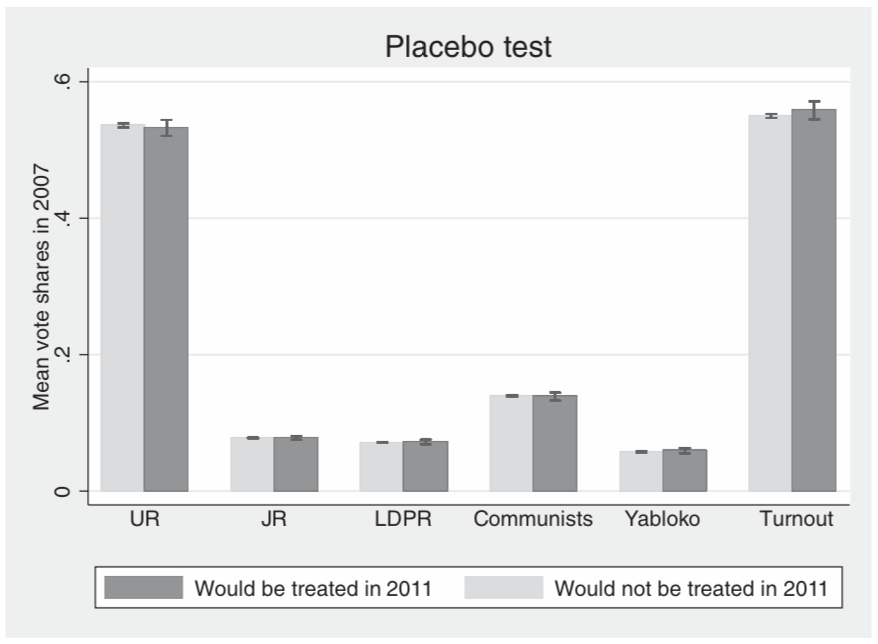
\includegraphics[width=\textwidth]{Images/placebo_test.png}
    \label{fig:my_label}
    
\end{figure}
\end{frame}


% \nocite{angrist2008mostly:3.2.1}



% PUSH THE WORDS ASSUMPTIONS AND POPPER VIEW ON THEM
% we will falsify always and have many strategies for falsification